\documentclass{beamer}
\usefonttheme[onlymath]{serif}
\usepackage[T1]{fontenc}
\usepackage[utf8]{inputenc}
\usepackage[english, icelandic]{babel}
\usepackage{amsmath}
\usepackage{amssymb}
\usepackage{amsthm}
\usepackage{gensymb}
\usepackage{parskip}
\usepackage{mathtools}
\usepackage{xfrac}
\usepackage{graphicx}
\usepackage{xcolor}
\usepackage{tikz}
\usetikzlibrary{calc}
\usepackage{verbatim}
\usepackage{multicol}
\usepackage{minted}
\parskip 0pt

\DeclareMathOperator{\lcm}{lcm}
\DeclareMathOperator{\diam}{diam}
\DeclareMathOperator{\dist}{dist}
\DeclareMathOperator{\ord}{ord}
\DeclareMathOperator{\Aut}{Aut}
\DeclareMathOperator{\Inn}{Inn}
\DeclareMathOperator{\Ker}{Ker}
\DeclareMathOperator{\trace}{trace}
\DeclareMathOperator{\fix}{fix}
\DeclareMathOperator{\Log}{Log}
\newcommand\floor[1]{\left\lfloor#1\right\rfloor}
\newcommand\ceil[1]{\left\lceil#1\right\rceil}
\newcommand\abs[1]{\left|#1\right|}
\newcommand\p[1]{\left(#1\right)}
\newcommand\sqp[1]{\left[#1\right]}
\newcommand\cp[1]{\left\{#1\right\}}
\newcommand\norm[1]{\left\lVert#1\right\rVert}
\renewcommand\qedsymbol{$\blacksquare$}
\renewcommand\Im{\operatorname{Im}}
\renewcommand\Re{\operatorname{Re}}

\usetheme{Madrid}

\title{Deila \& drottna og kvik bestun}
\subtitle{Fleiri lausnaraðferðir}
\author{Atli Fannar Franklín}
\date{\today}

\graphicspath{{myndir/}}

\AtBeginSection[] {
  \begin{frame}
    \frametitle{Efnisyfirlit}
    \tableofcontents[currentsection]
  \end{frame}
}


\begin{document}

\frame{\titlepage}

\section[Smá STL]{Smá STL}

\begin{frame}
\frametitle{Pairs}

\begin{itemize}

\item<1-> Í C++ býr pair<A, B> til par af einhverju af tagi A og B. Ná má í fyrra stakið með .first og seinna með .second. Raðað er fyrst m.t.t. fyrra staks og seinna staks svo ef fyrri eru jöfn.

\item<2-> Oft notum við pair<int,int> eða pair<long long, long long>

\end{itemize}

\end{frame}

\begin{frame}[fragile]
\frametitle{Custom sort}

\begin{itemize}

\item<1-> Hægt er að sorta hlut með custom sort með eftirfarandi hætti (hér erum við að bera saman pairs af ints eins og þau væru brot)

\item<2-> Einnig er hægt að láta sets, maps, priority queues o.s.frv. nota custom sort

\end{itemize}

\end{frame}

\begin{frame}[fragile]
\frametitle{Custom sort kóði}

\begin{minted}{c++}
#include<bits/stdc++.h>
using namespace std;
typedef pair<int,int> ii;

struct iicomp {
    bool inline operator()(const ii& a, const ii& b) {
        return a.first * b.second < b.first * a.second;
    }
}; 

int main() {
	vector<ii> a(20, ii(0, 0));
	sort(a.begin(), a.end(), iicomp());
	set<ii, iicomp> s;
	priority_queue<ii, vector<ii>, iicomp> pq;
}
\end{minted}

\end{frame}

\section[Deila \& Drottna]{Deila \& drottna}

\begin{frame}
\frametitle{Hvað er deila \& drottna?}

\begin{itemize}

\item<1-> Lausnaraðferð sem felur í sér að skipta vandamálinu niður í smærri hliðstæð vandamál

\item<2->  Útfærsla felur þá í sér endurkvæmt fall sem skoðar smærri og smærri hlutvandamál þar til að vandamálið sé nógu lítið til að auðvelt sé að finna lausnina

\item<3-> En hvað má leysa með þessum hætti?

\end{itemize}

\end{frame}

\begin{frame}
\frametitle{Dæmi um deila og drottna reiknirit}

\begin{itemize}

\item<1-> Binary search (lang \textbf{LANG} mikilvægast)

\item<2-> Röðunarreiknirit, t.d. quicksort og mergesort

\item<3-> Closest point pair í $\mathcal{O}(n\log(n))$

\item<4-> Strassen algorithm

\item<5-> Cooley-Tukey Fast Fourier Transform

\end{itemize}

\end{frame}

\begin{frame}
\frametitle{Hvað er binary search?}

\begin{itemize}

\item<1-> Segjum að við höfum samfellt fall $f$ og tölu $c$ þ.a. til séu einhver $a < b$ þannig að $f(a)$ og $f(b)$ séu sitt hvoru megin við $c$

\item<3-> Þá getum við kíkt hvort fallið sé fyrir ofan eða neðan í miðjunni og haldið áfram að leita í réttum helmingi

\end{itemize}

\only<2-> {
\begin{center}
\begin{tikzpicture}[domain=0:4]
    \draw[->] (-0.2,0) -- (4.2,0) node[right] {$x$};
    \draw[->] (0,-1.2) -- (0,4.2) node[above] {$y$};
    \draw[color=red] plot[id=c] function{2} 
        node[right] {$y = c$};
    \draw[color=blue] plot[id=poly] function{0.9 + 1.08333*x - 0.75*x**2 + 0.166667*x**3} 
        node[right] {$y = f(x)$};
    \node[below] at (0.7,-0.125) {$a$};
    \draw (0.7,0.125) -- (0.7,-0.125);
    \draw[dashed, gray] (0.7,0.125) -- (0.7, 4.2);
    \node[below] at (3.7,-0.125) {$b$};
    \draw (3.7,0.125) -- (3.7,-0.125);
    \draw[dashed, gray] (3.7,0.125) -- (3.7,4.2);
    \node<3>[below] at (2.2,-0.125) {$\frac{a+b}{2}$};
    \draw<3> (2.2,0.125) -- (2.2,-0.125);
    \draw<3>[dashed, gray] (2.2,0.125) -- (2.2,4.2);
    \node<4->[below] at (2.95,-0.125) {$\frac{\frac{a+b}{2}+b}{2}$};
    \draw<4-> (2.95,0.125) -- (2.95,-0.125);
    \draw<4->[dashed, gray] (2.95,0.125) -- (2.95,4.2);
\end{tikzpicture}
\end{center}}

\end{frame}

\begin{frame}
\frametitle{Af hverju er þetta svona nytsamlegt?}

\begin{itemize}

\item<1-> Þetta er mjög hratt! Ef billengdin okkar hefur lengd $L$ og fallið tekur $T(n)$ tíma að reikna finnum við svarið (eða nógu góða nálgun) í $\mathcal{O}(T(n)\log(L))$ tíma

\item<2-> Þetta á ekki bara við um föll. Ef við erum bara með \textit{eitthvað} sem vex samfellt (t.d. er einhalla) og við viljum finna núllstöð á, þá getum við einfaldað málið

\item<3-> Almennt er málið að við viljum finna minnstu/stærstu töluna sem eitthvað gildir um. Ef það að eitthvað gildi um töluna gefi að það gildi um allar tölur fyrir ofan/neðan hana er hægt að helmingunarleita að tölunni

\item<4-> Hvers vegna hjálpar þetta? Þá er búið að einfalda vandamálið úr 'Hver er minnsta slíka talan?' í 'Er þetta hægt fyrir töluna $x$?' sem er oft \textit{miklu} auðveldara að leysa

\end{itemize}

\end{frame}

\begin{frame}
\frametitle{Tökum dæmi}

\begin{itemize}

\item<1-> Við höfum einhverja punkta $0\leq x_1\leq\dots\leq x_n\leq 10^9$ sem eru staðsetningar á túristaíbúðum meðfram beinni strandlengju. Við höfum svo að $k \leq n$ túristar vilji leigja íbúð. Túristarnir vilja verða sem minnst varir við aðra túrista, svo við viljum hafa bilið milli túristanna sem búa næst hvoröðrum sem lengst. Hver er þessi hámarks stysta lengd?

\item<2-> Ef þetta er hægt með stystu lengd $r$ er þetta líka hægt fyrir styttri stystu lengd. Því helmingunarleitum við yfir stystu lengdina. Þá er spunringin orðin, er hægt að raða túristunum niður þannig að það sé a.m.k. $r$ langt milli þeirra allra?

\item<3-> Nú getum við gert restina gráðugt. Það er alltaf betra að setja túrista í hús á endunum og eins nálægt endunum og hægt er. Því setjum við bara túrista í húsið 'lengst til vinstri', svo næsta hús sem er a.m.k. $r$ í burtu o.s.frv. Þá ef við komum túristunum fyrir er svarið já fyrir $r$, annars nei. 

\end{itemize}

\end{frame}

\begin{frame}[fragile]
\frametitle{Lausnin}

\begin{scriptsize}
\begin{minted}{c++}
#include<bits/stdc++.h>
using namespace std;

int main() {
    long long n, k;
    cin >> n >> k;
    vector<long long> v(n);
    for(int i = 0; i < n; ++i) cin >> v[i];
    long long ans = 1, minans = 1, maxans = 10000000000;
    while(maxans - minans > 0) {
        long long pos = v[0], cnt = 1, midans = (maxans + minans) / 2;
        for(int i = 1; i < n; ++i) {
            if(v[i] - pos >= midans) cnt++, pos = v[i];
        }
        if(cnt < k) maxans = midans - 1;
        else ans = midans, minans = midans + 1;
    }
    cout << ans << endl;
    return 0;
}
\end{minted}
\end{scriptsize}

\end{frame}

\begin{frame}
\frametitle{Önnur deila og drottna reiknirit}

\begin{itemize}

\item<1-> Helmingunarleit er einfalt í útfærslu miðað við önnur deila og drottna reiknirit (þó svo að það að sjá út hvenær á að nota það getur verið erfitt)

\item<2-> Stundum þarf að skipta dæminu upp og skoða alla partana sem skipt er upp í og svo jafnvel að sameina lausnir í lokin

\item<3-> Þetta eru ekki rosa algeng dæmi, en gott er að þekkja til þeirra ef maður þarf að leysa dæmi með þessum hætti

\item<4-> Þó svo að það sé ekki beint keppnisforritunardæmi lýsir mergesort reikniritið þessu mjög vel, skoðum því mergesort snöggvast

\end{itemize}

\end{frame}

\begin{frame}
\frametitle{Mergesort}

\begin{itemize}

\item<1-> Mergesort felur það í sér að skipta lista í tvennt, kalla endurkvæmt á sjálft sig í báðum helmingum og sameina niðurstöður með því að sameina báða röðuðu listana í línulegum tíma

\only<2-> {
\begin{center}
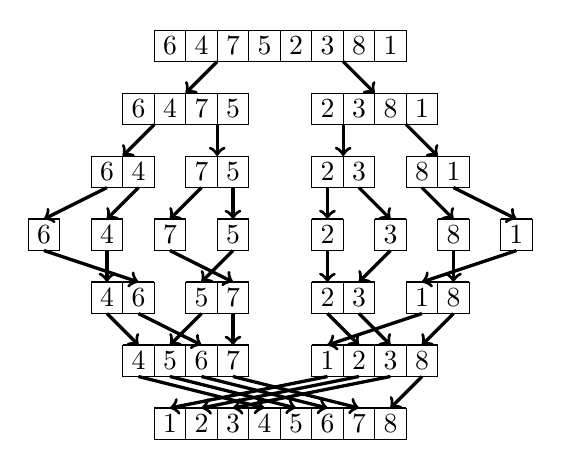
\begin{tikzpicture}[scale=0.4]
	\draw[step=1.0,black,thin] (0,8) grid (8,9);
	\node at (0.5,8.5) {$6$};
	\node at (1.5,8.5) {$4$};
	\node at (2.5,8.5) {$7$};
	\node at (3.5,8.5) {$5$};
	\node at (4.5,8.5) {$2$};
	\node at (5.5,8.5) {$3$};
	\node at (6.5,8.5) {$8$};
	\node at (7.5,8.5) {$1$};
	\draw[->, very thick] (2,8) -- (1,7);
	\draw[->, very thick] (6,8) -- (7,7);
	\draw[step=1.0,black,thin] (-1,6) grid (3,7);
	\draw[step=1.0,black,thin] (5,6) grid (9,7);
	\node at (-0.5,6.5) {$6$};
	\node at (0.5,6.5) {$4$};
	\node at (1.5,6.5) {$7$};
	\node at (2.5,6.5) {$5$};
	\node at (5.5,6.5) {$2$};
	\node at (6.5,6.5) {$3$};
	\node at (7.5,6.5) {$8$};
	\node at (8.5,6.5) {$1$};
	\draw[->, very thick] (0,6) -- (-1,5);
	\draw[->, very thick] (2,6) -- (2,5);
	\draw[->, very thick] (6,6) -- (6,5);
	\draw[->, very thick] (8,6) -- (9,5);
	\draw[step=1.0,black,thin] (-2,4) grid (0,5);
	\draw[step=1.0,black,thin] (1,4) grid (3,5);
	\draw[step=1.0,black,thin] (5,4) grid (7,5);
	\draw[step=1.0,black,thin] (8,4) grid (10,5);
	\node at (-1.5,4.5) {$6$};
	\node at (-0.5,4.5) {$4$};
	\node at (1.5,4.5) {$7$};
	\node at (2.5,4.5) {$5$};
	\node at (5.5,4.5) {$2$};
	\node at (6.5,4.5) {$3$};
	\node at (8.5,4.5) {$8$};
	\node at (9.5,4.5) {$1$};
	\draw[->, very thick] (-1.5,4) -- (-3.5,3);
	\draw[->, very thick] (-0.5,4) -- (-1.5,3);
	\draw[->, very thick] (1.5,4) -- (0.5,3);
	\draw[->, very thick] (2.5,4) -- (2.5,3);
	\draw[->, very thick] (5.5,4) -- (5.5,3);
	\draw[->, very thick] (6.5,4) -- (7.5,3);
	\draw[->, very thick] (8.5,4) -- (9.5,3);
	\draw[->, very thick] (9.5,4) -- (11.5,3);
	\draw[step=1.0,black,thin] (-4,2) grid (-3,3);
	\draw[step=1.0,black,thin] (-2,2) grid (-1,3);
	\draw[step=1.0,black,thin] (0,2) grid (1,3);
	\draw[step=1.0,black,thin] (2,2) grid (3,3);
	\draw[step=1.0,black,thin] (5,2) grid (6,3);
	\draw[step=1.0,black,thin] (7,2) grid (8,3);
	\draw[step=1.0,black,thin] (9,2) grid (10,3);
	\draw[step=1.0,black,thin] (11,2) grid (12,3);
	\node at (-3.5,2.5) {$6$};
	\node at (-1.5,2.5) {$4$};
	\node at (0.5,2.5) {$7$};
	\node at (2.5,2.5) {$5$};
	\node at (5.5,2.5) {$2$};
	\node at (7.5,2.5) {$3$};
	\node at (9.5,2.5) {$8$};
	\node at (11.5,2.5) {$1$};
	\draw[->, very thick] (-3.5,2) -- (-0.5,1);
	\draw[->, very thick] (-1.5,2) -- (-1.5,1);
	\draw[->, very thick] (0.5,2) -- (2.5,1);
	\draw[->, very thick] (2.5,2) -- (1.5,1);
	\draw[->, very thick] (5.5,2) -- (5.5,1);
	\draw[->, very thick] (7.5,2) -- (6.5,1);
	\draw[->, very thick] (9.5,2) -- (9.5,1);
	\draw[->, very thick] (11.5,2) -- (8.5,1);
	\draw[step=1.0,black,thin] (-2,0) grid (0,1);
	\draw[step=1.0,black,thin] (1,0) grid (3,1);
	\draw[step=1.0,black,thin] (5,0) grid (7,1);
	\draw[step=1.0,black,thin] (8,0) grid (10,1);
	\node at (-1.5,0.5) {$4$};
	\node at (-0.5,0.5) {$6$};
	\node at (1.5,0.5) {$5$};
	\node at (2.5,0.5) {$7$};
	\node at (5.5,0.5) {$2$};
	\node at (6.5,0.5) {$3$};
	\node at (8.5,0.5) {$1$};
	\node at (9.5,0.5) {$8$};
	\draw[->, very thick] (-1.5,0) -- (-0.5,-1);
	\draw[->, very thick] (-0.5,0) -- (1.5,-1);
	\draw[->, very thick] (1.5,0) -- (0.5,-1);
	\draw[->, very thick] (2.5,0) -- (2.5,-1);
	\draw[->, very thick] (5.5,0) -- (6.5,-1);
	\draw[->, very thick] (6.5,0) -- (7.5,-1);
	\draw[->, very thick] (8.5,0) -- (5.5,-1);
	\draw[->, very thick] (9.5,0) -- (8.5,-1);
	\draw[step=1.0,black,thin] (-1,-2) grid (3,-1);
	\draw[step=1.0,black,thin] (5,-2) grid (9,-1);
	\node at (-0.5,-1.5) {$4$};
	\node at (0.5,-1.5) {$5$};
	\node at (1.5,-1.5) {$6$};
	\node at (2.5,-1.5) {$7$};
	\node at (5.5,-1.5) {$1$};
	\node at (6.5,-1.5) {$2$};
	\node at (7.5,-1.5) {$3$};
	\node at (8.5,-1.5) {$8$};
	\draw[->, very thick] (-0.5,-2) -- (3.5,-3);
	\draw[->, very thick] (0.5,-2) -- (4.5,-3);
	\draw[->, very thick] (1.5,-2) -- (5.5,-3);
	\draw[->, very thick] (2.5,-2) -- (6.5,-3);
	\draw[->, very thick] (5.5,-2) -- (0.5,-3);
	\draw[->, very thick] (6.5,-2) -- (1.5,-3);
	\draw[->, very thick] (7.5,-2) -- (2.5,-3);
	\draw[->, very thick] (8.5,-2) -- (7.5,-3);
	\draw[step=1.0,black,thin] (0,-4) grid (8,-3);
	\node at (0.5,-3.5) {$1$};
	\node at (1.5,-3.5) {$2$};
	\node at (2.5,-3.5) {$3$};
	\node at (3.5,-3.5) {$4$};
	\node at (4.5,-3.5) {$5$};
	\node at (5.5,-3.5) {$6$};
	\node at (6.5,-3.5) {$7$};
	\node at (7.5,-3.5) {$8$};
\end{tikzpicture}
\end{center}}

\end{itemize}

\end{frame}

\begin{frame}[fragile]
\frametitle{Útfærsla}

\begin{tiny}
\begin{minted}{c++}
#include<bits/stdc++.h>
using namespace std;

void merge(int* a, int l, int m, int r) {
    int cnt1 = l, cnt2 = m + 1, cnt3 = 0;
    int acopy[r - l + 1];
    while(cnt1 <= m || cnt2 <= r) {
        if(cnt2 > r) acopy[cnt3] = a[cnt1++];
        else if(cnt1 > m) acopy[cnt3] = a[cnt2++];
        else if(a[cnt1] <= a[cnt2]) acopy[cnt3] = a[cnt1++];
        else acopy[cnt3] = a[cnt2++];
        cnt3++;
    }
    for(int i = l; i <= r; ++i) a[i] = acopy[i - l];
}

void mergesort(int* a, int l, int r) {
	if(r <= l) return;
	int m = l + (r - l) / 2;
	mergesort(a, l, m);
	mergesort(a, m + 1, r);
	merge(a, l, m, r);
}

int main() {
	int a[8] = {6, 4, 7, 5, 2, 3, 8, 1};
	mergesort(a, 0, 7);
	for(int i = 0; i < 8; ++i) cout << a[i] << ' ';
	cout << endl;
}
\end{minted}
\end{tiny}

\end{frame}

\section[Kvik bestun]{Kvik bestun}

\begin{frame}
\frametitle{Hvað er kvik bestun?}

\begin{itemize}

\item<1-> Það er í raun almennari útgáfa af deila og drottna

\item<2-> Við erum áfram að skipta vandamálinu niður í smærri vandamál en við geymum lausnirnar á smærri vandamálunum

\item<3-> Þetta þýðir að ef sama hlutvandamálið kemur upp oftar en einu sinni, þá erum við geymda lausn á því og þurfum ekki að reikna það aftur

\item<4-> Tökum (contrived) dæmi um þetta

\end{itemize}

\end{frame}

\begin{frame}

\begin{itemize}

\item<1-> Við viljum reikna $n$-tu Fibonnacci töluna, $f_n$. Hvernig má reikna hana?

\item<2-> Nú við vitum $f_n = f_{n-1} + f_{n - 2}$. Sjáum hvað gerist ef við reiknum þetta með deila og drottna.

\item<3-> Þá getum við sagt að ef það tekur $T(n)$ tíma að reikna $f_n$ þá gildi jafnan $T(n) = T(n-1) + T(n-2)$

\item<4-> Leysa má út úr þessu og fá að $T(n)$ sé $\mathcal{O}(2^n)$. Þetta er \textit{rosalega} hægt, við komumst varla upp í $f_{30}$

\item<5-> Hvert er vandamálið okkar? Hvernig má bæta þetta?

\end{itemize}

\end{frame}

\begin{frame}

\begin{center}
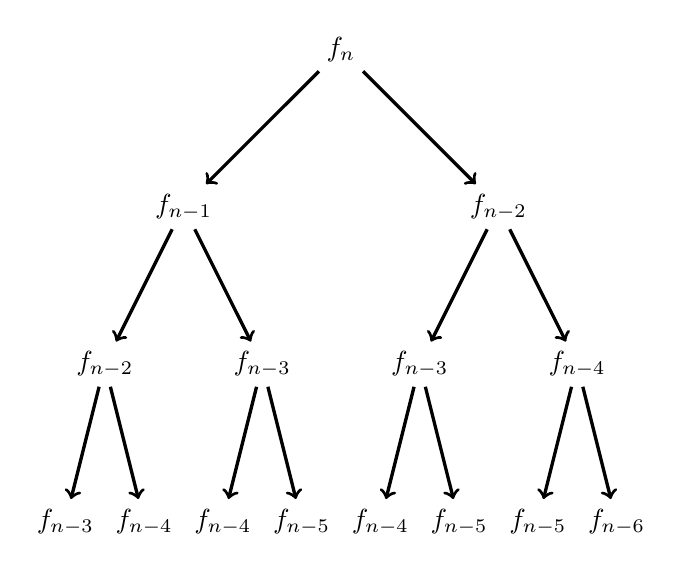
\begin{tikzpicture}

\node (n11) at (0,7) {$f_n$};
\node (n21) at (-2,5) {$f_{n-1}$};
\node (n22) at (2,5) {$f_{n-2}$};
\node (n31) at (-3,3) {$f_{n-2}$};
\node (n32) at (-1,3) {$f_{n-3}$};
\node (n33) at (1,3) {$f_{n-3}$};
\node (n34) at (3,3) {$f_{n-4}$};
\node (n41) at (-3.5,1) {$f_{n-3}$};
\node (n42) at (-2.5,1) {$f_{n-4}$};
\node (n43) at (-1.5,1) {$f_{n-4}$};
\node (n44) at (-0.5,1) {$f_{n-5}$};
\node (n45) at (0.5,1) {$f_{n-4}$};
\node (n46) at (1.5,1) {$f_{n-5}$};
\node (n47) at (2.5,1) {$f_{n-5}$};
\node (n48) at (3.5,1) {$f_{n-6}$};

\draw[->, very thick] (n11) -- (n21);
\draw[->, very thick] (n11) -- (n22);
\draw[->, very thick] (n21) -- (n31);
\draw[->, very thick] (n21) -- (n32);
\draw[->, very thick] (n22) -- (n33);
\draw[->, very thick] (n22) -- (n34);
\draw[->, very thick] (n31) -- (n41);
\draw[->, very thick] (n31) -- (n42);
\draw[->, very thick] (n32) -- (n43);
\draw[->, very thick] (n32) -- (n44);
\draw[->, very thick] (n33) -- (n45);
\draw[->, very thick] (n33) -- (n46);
\draw[->, very thick] (n34) -- (n47);
\draw[->, very thick] (n34) -- (n48);

\end{tikzpicture}
\end{center}

\end{frame}

\begin{frame}
\frametitle{Endurtekningar}

\begin{itemize}

\item<1-> Sjáum að við erum að reikna sömu töluna margoft

\item<2-> Því myndi þetta ganga miklu betur ef við geymdum tölurnar hingað til

\item<3-> Við búum til fylki $f[n]$ sem geymir $f_1,\dots,f_n$ og þá getum við reiknað hverja tölu $f_i$ í föstum tíma með því að leggja saman hinar tvær á undan í fylkinu

\item<4-> Þá er hægt að reikna þetta í $\mathcal{O}(n)$, sem er \textbf{miklu} hraðara!

\item<5-> Við komumst upp í $f_{10^8}$ án neinna vandræða, miklu betra en að ná varla $f_{30}$

\item<6-> Reyndar má reikna $f_n$ í $\mathcal{O}(\log(n))$ tíma. Þeir sem eru áhugasamir mega reyna pæla í því hvernig má gera það. Hint: Notið fylkjamargföldun

\end{itemize}

\end{frame}

\begin{frame}
\frametitle{LCS}

\begin{itemize}

\item<1-> Skoðum klassískt vandamál sem má leysa með kvikri bestun (og er besta slíka lausn)

\item<2-> Höfum tvær raðir af tölum $x_1,\dots,x_n$ og $y_1,\dots,y_m$ og viljum finna lengd lengstu runu af tölum $z_1,\dots,z_k$ sem er hlutruna í þeim báðum (LCS stendur fyrir Longest Common Subsequence)

\item<3-> Að prófa allar hlutrunur í þeim báðum og bera saman er $\mathcal{O}(\max(n, m)2^{\min(n, m)})$ sem er óhugnalega hægt

\item<4-> Notum kvika bestun! En hvernig á taflan okkar að líta út? Og hvernig skiptum við vandamálinu upp?

\end{itemize}

\end{frame}

\begin{frame}
\frametitle{LCS}

\begin{itemize}

\item<1-> Búum til töflu $T$ af stærð $nm$ og látum $T[i][j]$ vera lengd lengstu sameiginlegu hlutrunu $x_1,\dots,x_i$ og $y_1,\dots,y_j$

\item<2-> Sem grunntilvik er ljóst að $T[i][0] = T[0][j] = 0$ því allar hlutrunur í tómri runu eru tómar

\item<3-> Skoðum nú hvernig við getum reiknað $T[i][j]$. Ef $x_i = y_j$ þá er best að láta þau vera í hlutrununni, svo þá er $T[i][j] = T[i - 1][j - 1] + 1$. Ef $x_i \neq y_j$ geta þau ekki bæði verið í hlutrununni sem sameiginlegt stak, svo við þurfum að sleppa $x_i$ eða $y_j$. En þá fæst að $T[i][j] = \max(T[i - 1][j], T[i][j - 1])$.

\item<4-> Þar sem að reikna út $T[i][j]$ tekur fastan tíma gefur þetta þá af sér $\mathcal{O}(nm)$ lausn á vandamálinu!

\end{itemize}

\end{frame}

\begin{frame}[fragile]

\begin{scriptsize}
\begin{minted}{c++}
#include<bits/stdc++.h>
using namespace std;

int lcs(int* x, int n, int* y, int m) {
    int t[n + 1][m + 1];
    memset(t, 0, sizeof(t));
    for(int i = 1; i <= n; ++i) {
        for(int j = 1; j <= m; ++j) {
            if(x[i - 1] == y[j - 1]) {
                t[i][j] = t[i - 1][j - 1] + 1;
            } else {
                t[i][j] = max(t[i - 1][j], t[i][j - 1]);
            }
        }
    }
    return t[n][m];
}

int main() {
    int x[12] = {'a', 't', 'l', 'i', 'f', 'r', 'a', 'n', 'k', 'l', 'i', 'n'};
    int y[15] = {'b', 'e', 'r', 'g', 'u', 'r', \
        's', 'n', 'o', 'r', 'r', 'a', 's', 'o', 'n'};
    cout << lcs(x, 12, y, 15) << endl;
}
\end{minted}
\end{scriptsize}

\end{frame}

\begin{frame}
\frametitle{Keppnisforritunardæmi}

\begin{itemize}

\item<1-> Kvik bestunardæmi eru afar algeng í forritunarkeppnum

\item<2-> Eiginlega alla vega 2 af 10-12 dæmum um kvika bestun

\item<3-> Því er gott að æfa sig vel í að læra að hugsa um hvernig megi skipta dæminu upp og hvernig eigi að geyma hlutvandamálin í töflu

\item<4-> Skoðum því dæmi úr keppni og leysum það saman

\end{itemize}

\end{frame}

\begin{frame}
\frametitle{Shopaholic, erfiðari útgáfa}

\begin{itemize}

\item<1-> Fáum gefin $1 \leq n \leq 2000$ og $1 \leq d \leq 20$ og svo $n$ tölur $1 \leq p_1,\dots,p_n \leq 10000$. $p_i$-in eru vörunar okkar í þeirri röð sem við erum búin að raða þeim á vörubeltið. $d$ er fjöldi skiptibúta sem við erum með sem við getum lagt á vörubandið til að skipta kaupunum upp til að borga hlutina í stit hvoru lagi. Búðin rúnnar hlutina að næsta margfeldi af 10 krónum (5 upp á við). Hversu mikið þurfum við að borga fyrir vörurnar í minnsta lagi?

\item<2-> Hvernig töflu viljum við búa til? Hvernig viljum við reikna gildi töflunnar?

\end{itemize}

\end{frame}

\begin{frame}
\frametitle{Uppsetning töflu}

\begin{itemize}

\item<1-> Látum $T[i][j]$ vera hvað við þurfum að borga í minnsta lagi fyrir fyrstu $i$ vörurnar ef við höfum $j$ skiptibúta til umráða

\item<2-> Hver eru grunntilvik okkar? Ef $i = 0$ höfum við engar vörur svo $T[0][j] = 0$. Ef $j = 0$ er svarið bara hvað við þurfum að borga mikið fyrir fyrstu $i$ vörurnar. 

\item<3-> Hvað annars? Einhver skiptibútur þarf að vera lengst til hægri af öllum skiptibútum okkar. Því getum við ítrað yfir $k = 1,\dots,i$ og prófað að setja bútinn okkar sem er lengst til hægri þar. Ef við setjum hann þar er kostnaðurinn $T[k][j-1]$ fyrir það sem er vinstra megin við skiptibútinn en bara kostnaðurinn af restinni fyrir það sem er vinstra megin (því þar verða engir skiptibútar).

\end{itemize}

\end{frame}

\begin{frame}[fragile]
\frametitle{Lausnin}

\begin{tiny}
\begin{minted}{c++}
#include <bits/stdc++.h>
using namespace std;

int dp[2005][25];
int pref[2005];
int vals[2005];

int myround(int n) {
    return n % 10 < 5 ? n - (n % 10) : n - (n % 10) + 10;
}

int dplookup(int i, int j) {
    if(dp[i][j] != -1) return dp[i][j];
    if(i == 0) return dp[i][j] = 0;
    if(j == 0) return dp[i][j] = myround(pref[i - 1]);
    int mn = INT_MAX;
    for(int k = 0; k <= i; ++k) {
        mn = min(mn, dplookup(k, j - 1) + myround(pref[i - 1] - pref[k - 1]));
    }
    return dp[i][j] = mn;
}

int main() {
    int n, d;
    memset(dp, -1, sizeof(dp));
    cin >> n >> d;
    for(int i = 0; i < n; ++i) cin >> vals[i];
    pref[0] = vals[0];
    for(int i = 1; i < n; ++i) pref[i] = pref[i - 1] + vals[i];
    cout << dplookup(n, d) << endl;
}
\end{minted}
\end{tiny}

\end{frame}

\begin{frame}
\frametitle{Nokkur atriði varðandi kvika bestun}

\begin{itemize}

\item<1-> Í sjálfu sér er þetta kannski ekki flóknasta aðferðafræðin, en dæmi af þessari gerð má gera óguðlega erfið

\item<2-> Fyrsta sem benda má á er að það séu í raun tvær tegundir lausna, bottom-up og top-down

\item<3-> Í bottom up ítrum við einu sinni í gegnum töfluna og reiknum út öll gildin og sækjum svo svarið okkar (eins og við gerðum fyrir LCS)

\item<4-> Í bottom up getur röð lykkja skipt höfuðmáli (dæmi eftir smá)

\item<5-> Í top down búum við til hjálparfall sem sækir gildi í töfluna og reiknar það endurkvæmt með því að kalla í sjálft sig ef það er ekki búið að reikna gildið nú þegar

\item<6-> Það fer bara eftir aðstæðum hvort er þægilegra eða betra

\end{itemize}

\end{frame}

\begin{frame}
\frametitle{Lykkjuröð í bottom up}

\begin{itemize}

\item<1-> Gefum okkur eitthvað fylki $x$ af heiltölum. Skoðum hver munurinn er á að finna mögulegar summur þessarra talna þegar nota má sömu töluna oft og þegar nota má hverja tölu aðeins einu sinni.

\item<2-> Gerum fylki $dp$ þar sem $dp[i]$ er hvort rita megi $i$ sem summu af þessum tölum.

\item<3-> Sjáum nú tvær leiðir til að reikna út gildi $dp$ eftir því hvort endurtaka megi gildin eða ekki

\end{itemize}

\end{frame}

\begin{frame}[fragile]
\frametitle{Með endurtekningum}

\begin{minted}{c++}
#include <bits/stdc++.h>
using namespace std;

int main() {
    int x[4] = {1, 5, 13, 27};
    int dp[100];
    memset(dp, 0, sizeof(dp));
    dp[0] = 1;
    for(int i = 0; i < 4; ++i) {
        for(int j = 0; j < 100; ++j) {
            if(x[i] > j) continue;
            if(dp[j - x[i]] == 0) continue;
            dp[j] = 1;
        }
    }
    cout << dp[3] << endl; // prentar 1
}
\end{minted}

\end{frame}

\begin{frame}[fragile]
\frametitle{Án endurtekninga}

\begin{minted}{c++}
#include <bits/stdc++.h>
using namespace std;

int main() {
    int x[4] = {1, 5, 13, 27};
    int dp[100];
    memset(dp, 0, sizeof(dp));
    dp[0] = 1;
    for(int i = 0; i < 4; ++i) {
        for(int j = 100; j >= 0; --j) {
            if(x[i] > j) continue;
            if(dp[j - x[i]] == 0) continue;
            dp[j] = 1;
        }
    }
    cout << dp[3] << endl; // prentar 0
}
\end{minted}

\end{frame}

\begin{frame}
\frametitle{Sækja lausn}

\begin{itemize}

\item<1-> Stundum þarf að skila runu af tölum eða streng eða einhverskonar heila lausn í stað þess að skila bara tölu

\item<2-> T.d. skila hverjar skiptingarnar voru í cent savings eða hver lengsta sameiginlega runan er í LCS

\item<3-> Þá er oft gott að gera aðra töflu $L$ sem er jafnstór hinni töflunni $T$. Svo fyrir hvert gildi sem við setjum í $T$ setjum við í $L$ gildið sem við notuðum til að búa til lausnina í $T$

\item<4-> Þá getum við ítrað í gegnum $L$ til að fá lausnina okkar, tökum dæmi með summu talna eins og að ofan

\end{itemize}

\end{frame}

\begin{frame}[fragile]
\frametitle{Sækja lausn sýnidæmi}

\begin{scriptsize}
\begin{minted}{c++}
#include <bits/stdc++.h>
using namespace std;

int main() {
    int x[4] = {1, 5, 13, 27};
    int dp[100], last[100];
    memset(dp, 0, sizeof(dp));
    dp[0] = 1;
    for(int i = 0; i < 4; ++i) {
        for(int j = 99; j >= 0; --j) {
            if(x[i] > j || !dp[j - x[i]] || dp[j]) continue;
            dp[j] = 1, last[j] = i;
        }
    }
    int s = 41;
    cout << s << " = ";
    while(s > 0) {
        cout << x[last[s]];
        s -= x[last[s]];
        if(s != 0) cout << " + ";
    }
    cout << endl;
}
\end{minted}
\end{scriptsize}

\end{frame}

\end{document}